\section{Methods}\label{methods}

Fully dense neural network (NN) architectures, such as the one shown in Figure~\ref{fig:nn-1}, perform a sequence of affine transformations, ${\bold z}_i \leftarrow \boldsymbol\theta_i {\bold x}^{(i)}$, followed by element-wise functional operations, $\sigma({\bold z}_i)$ to introduce non-linearity at each layer; that is, each layer stretches and distorts the underlying space.
\begin{figure}[htbp]
\begin{center}
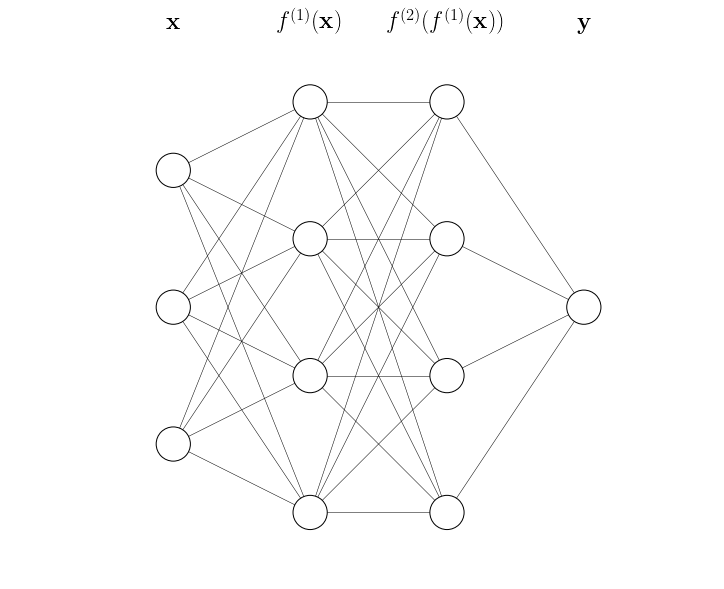
\includegraphics[width=0.4\textwidth]{fig/neural-network-01}
\caption{Schematic view of a fully dense neural network. Each sequence of affine and non-linear transformations are captured in the function, $f_i({\bold x}): {\bold x}^{(i+1)} \leftarrow \sigma(\boldsymbol\theta_i {\bold x}^{(i)})$}
\label{fig:nn-1}
\end{center}
\end{figure}

The resulting network,
\begin{equation}
	f(x) = \sigma(\boldsymbol\theta_n \sigma(\boldsymbol\theta_{n-1} \sigma(\ldots \boldsymbol\theta_2 \sigma(\boldsymbol\theta_1{\bold x}))))
	\label{eqn:nn analytical form}
\end{equation}
is an arbitrary function generator, but at present, the network weights $\boldsymbol\theta_i$ can not map back to analytic forms that capture and describe the underlying physics. There are, however, many such mappings through polynomial series expansions,
\begin{equation}
	f(x) = \sum_{n=0}^\infty a_n x^n
\end{equation}

We hypothesize that the physics of a process can be extracted by fitting the polynomial expansions of known physical relationships to the polynomial coefficients of a polynomial series expansion of Equation~(\ref{eqn:nn analytical form}). \\
\\*

The ReLU function is given below in Equation~(\ref{eqn:ReLU}):
\begin{equation}
	f(x) = 
	\begin{cases}
		x, & \text{if}\ x > 0 \\
		0, & \text{otherwise}
	\end{cases}
	\label{eqn:ReLU}
\end{equation}

\begin{equation}
	f(x) = \sigma(\theta_n \sigma(\theta_{n-1} \sigma(\ldots \theta_2 \sigma(\theta_1 x))))
\end{equation}
\\
The variable $\boldsymbol x$ represents a column vector containing $\boldsymbol n$ elements, and thus, the output from each node will be multplied by the respective weight, $\theta$, before the application of the subsequent acitivation function. \\*

e.g., 
\begin{equation}
	\sigma_2 \begin{bmatrix}
				x_{1} \\
				x_{2} \\
				\vdots \\
				x_{n}
			\end{bmatrix}
	\Rightarrow \begin{bmatrix}
					\sigma_{11} x_{1} & \sigma_{12} x_{2} & \ldots & \sigma_{1n} x_{n} \\ 
					\sigma_{21} x_{1} & \sigma_{22} x_2 \\
					\vdots & & \ddots \\
					\sigma_{n1} x_{1} \\
				\end{bmatrix}			
\end{equation}


Although ReLU (rectified linear units) have become a more common activation function, its discontinuity at $x = 0$ requires an infinite series to fully capture the behavior at this transition. However, the softplus function,%However, the sigmoid function,
%\begin{equation}
%	\sigma(x) = \frac{1}{1 + e^{-x}}
%	\label{eqn:sigmoid}
%\end{equation}
%is a special case of the generating function for the Euler polynomial coefficients,
%\begin{equation}
%	\frac{2e^{x t}}{1 + e^t} = \sum_{n=0}^\infty E_n(x) \frac{t^n}{n!}
%\end{equation}
%where, for $x = 0$,
%\begin{equation}
%	\sigma(x) = \frac{1}{2} \sum_{n=0}^\infty E_n(0) \frac{(-1)^n}{n!}.
%	\label{eqn:sigmoid Euler expansion}
%\end{equation}
%
%The Euler polynomials at $x=0$,
%\begin{equation}
%	E_n(0) = -2(n+1)^{-1} \left( 2^{n+1} - 1 \right) B_{n+1}
%\end{equation}
%where $B_n$ is the $n^\textrm{th}$ Bernoulli number. Since Bernoulli numbers of odd index, with the exception of $B_1$, are zero, $E_i(0) = 0$ for $i = 2, 4, 6, \ldots, 2n$. Therefore, the summand and limits of Equation~(\ref{eqn:sigmoid Euler expansion}) change to
%\begin{equation}
%	\sigma(x) = \frac{1}{2} - \frac{1}{2} \sum_{n=1}^\infty \left( \frac{E_{2n-1(0)}}{(2n-1)!} \right) x^{2n-1}.
%\end{equation}
%
%The series representation of $E_{2n-1}(x)$
%\begin{equation}
%	E_{2n-1}(x) = \frac{(-1)^n 4 (2n - 1)!}{\pi^{2n+1}} \sum_{k=0}^\infty \frac{\cos [(2k + 1) \pi x]}{(2k + 1)^{2n}}
%\end{equation}
%such that,
%\begin{equation}
%	E_{2n-1}(0) = \frac{(-1)^n 4 (2n - 1)!}{\pi^{2n+1}} \sum_{k=0}^\infty \frac{1}{(2k + 1)^{2n}}
%\end{equation}
%and therefore,
%\begin{eqnarray}
%	\sigma(x) & = & \frac{1}{2} - \sum_{n=1}^\infty 2 \frac{(-1)^n}{\pi^{2n}} \left( \sum_{k=0}^\infty \frac{1}{(2k+1)^{2n}} \right) x^{2n-1} \\
%		& = & \frac{1}{2} - \sum_{n=1}^\infty 2 \frac{(-1)^n}{\pi^{2n}} \left( 4^{-n} \left( 4^n - 1 \right) \zeta(2n) \right) x^{2n-1} \nonumber \\
%		& = & \frac{1}{2} - \sum_{n=1}^\infty \underbrace{2 \left( \frac{-1}{4\pi^2} \right)^n \left( 4^n - 1 \right) \zeta(2n)}_{a_n} x^{2n-1} \nonumber \\
%		& = & \sum_{n=0}^\infty a_n x^n,\ a_n = \left\{ \begin{array}{l l}
%			1/2	& n = 0 \\
%			-2 \left( \frac{-1}{4\pi^2} \right)^{(n+1)/2} \left( 4^{(n+1)/2} - 1 \right)\zeta(n+1)	& n\ \text{odd} \\
%			0	& n\ \text{even}
%		\end{array}\right.
%		\label{eqn:sigmoid zeta expansion}
%\end{eqnarray}

\begin{equation}
	f(x) = log(1+e^x)
\end{equation}

The series expansion for the exponential
\begin{equation}
	e^x = \sum_{k=0}^\infty \frac{x^k}{k!}
\end{equation}
where, $a_k = \frac{1}{k!}$, can be expressed as
\begin{equation}
	e^x = \sum_{k=0}^\infty x^k a_k
\end{equation}

A similar series expansion for the logarithm
\begin{equation}
	log(1+x) = \sum_{n=1}^\infty (-1)^{n+1} \frac{x^n}{n}
\end{equation}
where, $x = e^x$,
allows for the softplus function to be represented as
\begin{equation}
	f(x) = \sum_{n=1}^\infty \frac{(-1)^{n+1}}{n} 				(\sum_{k=0}^\infty x^k a_k)^n
\end{equation}

If the expansion of $e^x$ is performed, then it can be seen that
\begin{equation}
	(\sum_{k=0}^\infty x^k a_k)^n = 								(a_0+x(a_1+x(a_2+xa_3...)))^n
\end{equation}

Using the binomial theorem
\begin{equation}
	(a+b)^n = \sum_{m=0}^{n} \binom{n}{m} a^{n-m} b^m
\end{equation}
where, $a=a_0$ and $b=(x(a_1+x(a_2+xa_3...)))^n$, the series expansion of the exponential can be represented as
\begin{equation}
	(\sum_{k=0}^\infty x^k a_k)^n = \sum_{m=0}^{n} 				\binom{n}{m} a_0^{n-m} (a_1+x(a_2+xa_3...))^n x^n
\end{equation}

Continuing with this approach, it can be seen that ...

% %%%%%%%%%%%%%%%%%%%%%%%%%%%%%%%%%%%%%%%%%%%%%%%%%%%%%%%%%%%%%%%%%%%%%%%%%%%%
The analytical form, combining Equations~(\ref{eqn:nn analytical form}) and (\ref{eqn:sigmoid zeta expansion}), the estimated output of a two-layer NN can be written as an expansion:

\begin{eqnarray}
	{\bold y}_1 & = & \sum_{k=0}^\infty a_k (\boldsymbol\theta_1^T {\bold x})\he{k} \nonumber \\
	{\bold y}_2 & = & \sum_{k=0}^\infty b_k (\boldsymbol\theta_2^T {\bold y}_1)\he{k} \nonumber \\
		& = & b_0 {\bold 1} + \nonumber\\
		&   & + b_1 (\tilde a_0 +%
					(\tilde a_1 + %
						(\tilde a_2 + %
							(\tilde a_3 + %
								(\ldots) \tilde {\bold x} )%
							\tilde {\bold x} )%
						\tilde {\bold x} )%
					\tilde {\bold x}) \nonumber \\
		&   & + b_2 (\tilde a_0 +%
					(\tilde a_1 + %
						(\tilde a_2 + %
							(\tilde a_3 + %
								(\ldots) \tilde {\bold x} )%
							\tilde {\bold x} )%
						\tilde {\bold x} )%
					\tilde {\bold x})^2 \nonumber \\
		&   & \vdots \nonumber \\
		&   & + b_k (\tilde a_0 +%
					(\tilde a_1 + %
						(\tilde a_2 + %
							(\tilde a_3 + %
								(\ldots) \tilde {\bold x} )%
							\tilde {\bold x} )%
						\tilde {\bold x} )%
					\tilde {\bold x})^k \nonumber \\
		&   & \vdots
\end{eqnarray}
\noindent where $\tilde a_i = \boldsymbol\theta_2^T a_i$ and $\tilde{\bold x} = \boldsymbol\theta_1^T {\bold x}$. All $\boldsymbol\theta_i$, ${\bold x}$, and ${\bold y}$ are augmented to include the bias, ${\bold b}_i$, that is,
\begin{eqnarray}
	{\bold x}&:& {\bold x} \leftarrow \begin{pmatrix}
								1 \\
								{\bold x}
							\end{pmatrix} = \begin{pmatrix}
											1 \\
											x_0 \\
											x_1 \\
											\vdots \\
											x_n
										\end{pmatrix}\\
	{\bold y}&:& {\bold y} \leftarrow \begin{pmatrix}
								1 \\
								{\bold y}
							\end{pmatrix} \\
	\boldsymbol\theta_i&:& \boldsymbol\theta_i \leftarrow \begin{pmatrix} {\bold b}_i & \boldsymbol\theta_i \end{pmatrix}
\end{eqnarray}

The element-wise exponent operator, ${\bf x}\he{m} = (x_1^m\ x_2^m\ \cdots\ x_n^m)^T$, raises each element of a vector or matrix to the specified power, $m$.

From Equation~(\ref{eqn:sigmoid zeta expansion}), $a_i  = 0\ \text{for}\ i = 2, 4, 6, \ldots$, and therefore,
\begin{align}
	{\bold y}_1 =& \sum_{k=0}^\infty a_k (\boldsymbol\theta_1^T {\bold x})\he{k} \nonumber \\
	{\bold y}_2 =& \sum_{k=0}^\infty b_k (\boldsymbol\theta_2^T {\bold y}_1)\he{k} \nonumber \\
		=& b_0 {\bold 1} + \nonumber\\
		 &+ b_1 (\tilde a_0 +%
					(\tilde a_1 + %
						(\tilde a_3 + %
							(\tilde a_5 + %
								(\ldots) \tilde {\bold x}\he{2} )%
							\tilde {\bold x}\he{2} )%
						\tilde {\bold x}\he{2} )%
					\tilde {\bold x}) \nonumber \\
		&+ b_2 (\tilde a_0 +%
					(\tilde a_1 + %
						(\tilde a_3 + %
							(\tilde a_5 + %
								(\ldots) \tilde {\bold x}\he{2} )%
							\tilde {\bold x}\he{2} )%
						\tilde {\bold x}\he{2} )%
					\tilde {\bold x})\he{2} \nonumber \\
		& \vdots \nonumber \\
		& + b_k (\tilde a_0 +%
					(\tilde a_1 + %
						(\tilde a_3 + %
							(\tilde a_5 + %
								(\ldots) \tilde {\bold x}\he{2} )%
							\tilde {\bold x}\he{2} )%
						\tilde {\bold x}\he{2} )%
					\tilde {\bold x})\he{k} \nonumber \\
		& \vdots \nonumber \\
	{\bold y}_2 = & \sum_{N=0}^\infty \sum_{k=0}^{N} \sum_{l=0}^{k} \sum_{m=0}^{l} \ldots %
		b_N %
		\binom{N}{k,l,m,\ldots} %
		\tilde a_0^k \tilde a_1^l \tilde a_3^m \ldots %
		\tilde {\bold x}\he{(N-k\ldots)} %
		({\tilde {\bold x}^2})\he{(N-k-l\ldots)} %
		({\tilde {\bold x}^2})\he{(N-k-l-m\ldots)} \nonumber \\
	 =& \sum_{N=0}^\infty \sum_{k=0}^{N} \sum_{l=0}^{k} \sum_{m=0}^{l} \ldots %
		b_N %
		\binom{N}{k,l,m,\ldots} %
		\tilde a_0^k \tilde a_1^l \tilde a_3^m \ldots %
		\tilde {\bold x}\he{(l+m+n+\ldots)} %
		({\tilde {\bold x}\he{2}})\he{(m+n+\ldots)} %
		({\tilde {\bold x}\he{2}})\he{(n+\ldots)}
	\label{eqn:ANN power series coefficient generating function}
\end{align}
\noindent where $k+l+m+n+\ldots = N$. Collecting coefficients and terms of power $k$,
\begin{equation*}
	{\bold y_2} =  \sum_{k=0}^\infty c_k \tilde{\bold x}\he{k}
\end{equation*}
\noindent that, having the same form as Equation~(\ref{eqn:sigmoid zeta expansion}) creates a sequential process for determining the coefficients of the power series expansion of each layer in an ANN. Importantly, the output layer in a ANN regression is a single node with a linear activation, so the final layer, $y_f$, working from the last hidden layer, ${\bold y}_n$, is simply,
\begin{equation}
	y_f = \boldsymbol\theta_n^T {\bold y}_n
\end{equation}
